\documentclass[xcolor=dvipsnames, compress]{beamer}
\usetheme[compress]{Madrid}
\setbeamertemplate{enumerate items}[square]
\setbeamertemplate{headline}{}
\setbeamertemplate{footline}
{
  \leavevmode%
  \hbox{%
  \begin{beamercolorbox}[wd=.4\paperwidth,ht=2.25ex,dp=1ex,center]{author in head/foot}%
    \usebeamerfont{author in head/foot}\insertshortauthor
  \end{beamercolorbox}%
  \begin{beamercolorbox}[wd=.6\paperwidth,ht=2.25ex,dp=1ex,center]{title in head/foot}%
    \usebeamerfont{title in head/foot}\insertshorttitle\hspace*{3em}
    \insertframenumber{} / \inserttotalframenumber\hspace*{1ex}   
  \end{beamercolorbox}}%
  \vskip0pt%
}
\usepackage{pgfplots}
\usepackage{pgfpages}
\usepackage[export]{adjustbox}
\usepackage[utf8]{inputenc}
%\setbeameroption{show notes on second screen}
\usepackage[outline]{contour}
\usepackage{transparent}
\usepackage{multimedia}
\usepackage{graphicx}
\usepackage{amsmath,amssymb}
\usepackage{bm}
\usepackage[absolute,overlay]{textpos}
\usepackage{mathtools}
\usepackage{courier}
\usepackage{tikz}
\tikzstyle{every picture}+=[remember picture]
\usetikzlibrary{positioning}
\usetikzlibrary{math}
\usetikzlibrary{arrows.meta}
\usepackage{caption}
\usepackage{lmodern}
\usepackage{tcolorbox}
\usepackage{xparse}
\tcbuselibrary{breakable,minted,xparse,skins,listings}
\usepackage[absolute,overlay]{textpos}

\beamertemplatenavigationsymbolsempty
\usefonttheme[onlymath]{serif}
\graphicspath{{./gfx/}}
\newcommand{\ppos}{q}
\newcommand{\pvel}{u}
\newcommand{\fpos}{r}
\newcommand{\fvel}{v}
\newcommand{\corr}{\text{corr}}
\newcommand{\dpr}{\text{\tiny DP}}
\newcommand{\qtd}{\text{\tiny q2D}}
\renewcommand{\vec}[1]{\bm{#1}}
\newcommand{\tens}[1]{\bm{\mathcal{#1}}}
\newcommand{\oper}[1]{\mathcal{#1}}
\newcommand{\uammd}{\gls{UAMMD}\xspace}
\newcommand{\gpu}{\gls{GPU}\xspace}
\newcommand{\dt}{\delta t}
\newcommand{\kT}{k_B T}
\newcommand{\sinc}{\textrm{sinc}}
\newcommand{\floor}{\textrm{floor}}
\newcommand{\near}{\textrm{near}}
\newcommand{\far}{\textrm{far}}
\newcommand{\half}{\frac{1}{2}}
\newcommand{\red}[1]{{\color{red}#1}}
\newcommand{\fou}[1]{\widehat{#1}}
\newcommand{\noise}{\widetilde{W}}

\newcommand{\executeiffilenewer}[3]{
  \ifnum
  \pdfstrcmp{\pdffilemoddate{#1}}{\pdffilemoddate{#2}}>0
  {\immediate\write18{#3}}
  \fi
}
\newcommand{\includesvg}[2][width=\columnwidth]{
  \executeiffilenewer{#2.svg}{#2.pdf}
  {inkscape -D #2.svg --export-type=pdf } %  --export-latex}
  \includegraphics[#1]{#2.pdf}
}



\def\ucpp{uammd_cpp_lexer.py:UAMMDCppLexer -x}
\usemintedstyle{default}
\setminted[\ucpp]{ %
  linenos=false,             % Line numbers
  autogobble=true,          % Automatically remove common white space
  fontsize=\small,
  breaklines
}
\AtBeginDocument{
  \newtcblisting{code2}[2][]{
    colback=white,
    colbacktitle=white,
    coltitle=black,
    pad at break*=0mm,
    listing only,
    listing engine=minted,
    listing remove caption=true,
    title={~#1},
    minted language=\ucpp,
    enhanced jigsaw,
    minipage boxed title,
    attach boxed title to bottom center={xshift=0mm,yshift=-1mm},
    boxed title style={size=small, blanker},
    center title,
    #2
  }
}

\AtBeginDocument{
  \newtcblisting{codebash}[2][]{
    colback=white,
    colbacktitle=white,
    coltitle=black,
    pad at break*=0mm,
    listing only,
    listing engine=minted,
    listing remove caption=true,
    title={~#1},
    minted language=shell,
    enhanced jigsaw,
    minipage boxed title,
    attach boxed title to bottom center={xshift=0mm,yshift=-1mm},
    boxed title style={size=small, blanker},
    center title,
    #2
  }
}
\tcbsetforeverylayer{autoparskip}

\title{Complex fluids in the GPU era}
\subtitle{Algorithms and simulations}
\author{Raúl P. Peláez}
\institute{Universidad Autónoma de Madrid}
\date{May 9, 2022}
%\captionsetup[figure]{font=small,skip=0pt}
\setbeamertemplate{itemize subitem}{$\rightarrow$}
%\pdfmapfile{-mpfonts.map}
\everymath{\displaystyle}
\begin{document}
\begin{frame}
  \titlepage
  \centering
\small  Supervisor: Rafael Delgado-Buscalioni
  \begin{figure}
    \centering
    \includegraphics[width=0.25\linewidth]{UAMlogo}
  \end{figure}
  \note{
    \begin{itemize}
    \item My work during these past years has been devoted to exploiting the GPU for the simulation of complex fluids.
    \item This is a GPU. A powerful hardware with a unique programming model.
    \item Harvesting its tremendous raw power requires developing algorithms and software specifically tailored for it.
    \item Now, before we start, let me give you a summary of this talk.
    \end{itemize}
  }
\end{frame}

\section{Introduction}
\begin{frame}
  \frametitle{Talk outline}
    \tableofcontents[
    sectionstyle=show/show,
    subsectionstyle=hide/hide/hide,
    subsubsectionstyle=hide/hide/hide/hide
    ]
\end{frame}

\subsection{Complex fluids}
\begin{frame}
  \frametitle{Complex fluids}
\centering \Large  The coexistence between a liquid and solid phase
  \begin{figure}
    \centering
    \includegraphics[width=0.5\linewidth]{membrane}\includegraphics[width=0.2\linewidth]{star}
    \includegraphics[width=0.2\linewidth]{optofluidics}\\
    {\fontsize{4.5}{12} \selectfont [{\bf Panzuela, S. and Delgado-Buscalioni, R.} PRL 2018.]  -  [{\bf Raul P. Pelaez and Delgado-Buscalioni, R.} Macromolecules 2020]    -   [{\bf  Mel\'endez, M.} et. al. PRE 2019.]}\\
    \only<1>{\movie[autostart,loop,poster,showcontrols=true,width=0.3\linewidth]{\includegraphics[width=0.3\linewidth]{virus_scr.png}}{gfx/virus.mp4}}%
    \only<2>{\includegraphics[width=0.235\linewidth]{lipostrandspablo.png}}%
    \movie[autostart,loop,poster,showcontrols=true,width=0.3\linewidth]{\includegraphics[width=0.3\linewidth]{rots.png}}{gfx/rots.mp4}%
    \only<1>{%
      \includegraphics[width=0.3\linewidth]{q2Dcolorstripe}\\
      {\fontsize{4.5}{12} \selectfont [Courtesy of Pablo Ibañez] ------------ [Courtesy of Berta Tinao] -------------- [{\bf Raul P. Pelaez} et. al. JSTAT 2018.]}%
    }
    \only<2>{%
      \includegraphics[width=0.22\linewidth]{mnppablo.png}\\
      {\fontsize{4.5}{12} \selectfont [Courtesy of Pablo Palacios] ------------------------ [Courtesy of Berta Tinao] ----------------------------------------- [Courtesy of Pablo Palacios]}
    }
  \end{figure}
  \note<1>{
    \scriptsize
    \begin{itemize}
    \item I showed you what a GPU is at the start. In order to understand the rest of the title you also need to know what a complex fluid is.
    \item Although its definition is a little more general, we understand a complex fluids as the coexistence between a solid and a liquid phase. And note that with solid, we usually mean soft, such as a colloidal particle or a cell's lipidic membrane.
    \item This broad definition encloses a wide variety of systems, many times of biological nature. In this slide I show you a bunch of examples, all of them taken from past and ongoing works in our group.
    \item Starting up we can see coarse-grained representations of a lipid bilayer, a star polymer under shear flow, a nano dumbell swimming and spinning in a fluid under optically-induced vortexes.
    \item A virus capsid, filled with a particular protein, which is being pressed by an AFM tip. Next we have a group of lipidic vesicles, one of them contains a ferromagnetic particle subjected to a magnetic field, spinning the vesicle. This allows to somewhat control the locomotion of the vesicles. The final picture shows the diffusion of the concentration of a colloidal suspension under strong two-dimensional confinement in different regimes.
    \end{itemize}    
  }  
  \note<2>{
    \begin{itemize}
    \item Here, the figure to the right shows a model of the rotating vesicles a member of group, Pablo, is studying now, in part using the tools and algorithms that I will shortly introduce.
    \item Pablo has also studied other kinds of magnetic nanoparticles.
    \item These examples showcase enormous span of the spatio-temporal scales associated with complex fluids. Sometimes we need to focus on single polymers, or describe a single protein in detail. Other times we want to model vesicles that are almost visible to the naked eye.
    \end{itemize}
  }
\end{frame}


\subsubsection{Numerical techniques}
\begin{frame}
  \frametitle{Complex fluids}
  \framesubtitle{The spatio-temporal landscape of numerical techniques.}
  \begin{figure}
    \centering
    \begin{tikzpicture}
      \only<1-5>{\node[anchor=south west, inner sep=0] (image) {\includesvg[width=0.8\linewidth]{gfx/landscape}};}
      \begin{scope}[shift={(image.south west)},x={(image.south east)},y={(image.north west)}]
        %\draw foreach \xy in {0,0.1,...,1.001}{(\xy,0) -- node[pos=0,below]{\pgfmathprintnumber{\xy}} (\xy,1)(0,\xy) -- node[pos=0,left]{\pgfmathprintnumber{\xy}} (1,\xy)};
        \only<2>{\filldraw[red, opacity=0.6] (0.12,1) rectangle (0.5,0.07) node[midway] (A) {};\node[above=50pt of A, black]{\contourlength{1pt}\contour{white}{\textbf{Fully Lagrangian}}};}
        \only<4>{\filldraw[blue, opacity=0.6] (0.5,1) rectangle (0.72,0.07) node[midway] (A) {};\node[below=40pt of A, black, align=left]{\contourlength{1pt}\contour{white}{\textbf{Immersed}}\\\contourlength{1pt}\contour{white}{\textbf{Boundary}}}; \node[above=30pt of A, black, align=left]{\contourlength{1pt}\contour{white}{\textbf{Eulerian}}\\\contourlength{1pt}\contour{white}{\textbf{Lagrangian}}};}
        \only<3>{\filldraw[green, opacity=0.6] (0.72,1) rectangle (1,0.07) node[midway] (A) {};\node[above=50pt of A, black]{\contourlength{1pt}\contour{white}{\textbf{Fully Eulerian}}};}
      \end{scope}
    \end{tikzpicture}
    \caption{Figure courtesy of Rafael Delgado-Buscalioni.}
  \end{figure}
  \note<1>{
    \begin{itemize}
    \item The modeling and simulation of complex fluids thus greatly exceeds the scope of the typical computation window. Speaking in terms of this numerical landscape we cannot specialize in a single window. If we want to model a complex fluid, we must take into account sizes ranging from nanometers to meters and times going from nanoseconds to seconds. And even then, we are restricted to a narrow-ish area of the lanscape, being unable to, for instance, simulate a nanometer-sized system for several hours of physical time.
    \item I claim that my software, UAMMD, covers the whole range of the complex-fluid domain, and I hope to convince you during this talk that this is true.
    \item Anyway, countless numerical and mathematical techniques exists depending on our window of interest, and their naming scheme can sometimes be a little obtuse.      
    \end{itemize}
  }
  \note<2>{
    \begin{itemize}
    \item Broadly speaking, we can categorize the landscape into three families of methods.
    \item When studying small systems, we usually choose a fully Lagrangian scheme, meaning that we track the evolution of individual particles, or markers.
    \end{itemize}
  }
  \note<3>{
    \begin{itemize}
    \item On the contrary, when focusing on macroscopic systems we usually choose a fully Eulerian description, where we loose track of individual particles and instead describe continuous fields.      
    \end{itemize}
  }
  \note<4>{
    \begin{itemize}
    \item In the middle, in what we call the mesoscale, there is a mixed domain of Eulerian-Lagrangian methods, where we describe both a group of particles and continuous fields that are somehow coupled.
    \item The Immersed boundary method is the canonical strategy used to describe this coupling.
    \item This is the realm of hydrodynamics, where most of the examples I showed you take place.
    \item I would like to point out now that my algorithmic contributions lie in this regime.
    \end{itemize}
  }
  \note<5>{
    \begin{itemize}
    \item Let us focus in the red area, covering an, in principle, disparate range of descriptions all related to complex fluids.
    \item If we start at the atomic scale and want to climb up the spatio-temporal scale of modeling we can make use of coarse graining techniques, where we want to somehow average out the fast degrees-of-freedom that are of no interest to us. For instance, if we are describing a submarine running under the sea (by all means a complex fluid) we really want to leave the individual water atoms out of our description.
    \end{itemize}
    }
\end{frame}

\subsubsection{Coarse-grained levels of description}
\begin{frame}
  \frametitle{Complex fluids}
  \framesubtitle{Usual levels of coarse-grained description}
  \begin{figure}
    \centering
    \includesvg[width=0.55\linewidth]{gfx/multiscale}
  \end{figure}
  \note{
    In particular, we can cover the whole range using the following four levels of coarse-grained description. Going through them will help us understand how we can design a framework that covers them all.
    }
\end{frame}


\begin{frame}[t]
  \frametitle{Complex fluids}
  \framesubtitle{Usual levels of coarse-grained description}
  \begin{columns}[T]
    \begin{column}{0.5\linewidth}
        \begin{tikzpicture}
          \node[anchor = south west, inner sep = 0] (image) {\includesvg[width=\linewidth]{gfx/multiscale}};
          \begin{scope}[shift={(image.south west)},x={(image.south east)},y={(image.north west)}]
            %Draw a overlaying grid to easily see where the rectangles must be, this can be commented out in the final version
%            \draw foreach \xy in {0,0.1,...,1.001}{
%            (\xy,0) -- node[pos=0,below]{\pgfmathprintnumber{\xy}} (\xy,1)
%            (0,\xy) -- node[pos=0,left]{\pgfmathprintnumber{\xy}} (1,\xy)};
            \foreach[count=\i] \mypath in {
              {(0,1) rectangle (0.48,0.55)},
              {(0.48,1) rectangle (1.0,0.55)},
              {(0,0.55) rectangle (0.48,0)},
              {(0.48,0.55) rectangle (1,0)},
              {(0,1) rectangle (1,0)},
              {(0,1) rectangle (1,0)}
            }{
              \filldraw<\i>[white,opacity=0.9,even odd rule] (0,0) rectangle (1,1) \mypath;
            }
          \end{scope}
        \end{tikzpicture}
      \end{column}
      \begin{column}{0.45\linewidth}
      \begin{center}
        \textbf{Relevant variables:}
      \end{center}
      \begin{itemize}
      \item<1-> $\vec{q}_i$: Position of particle $i$.
      \item<1-3,5-> $\vec{u}_i$: Velocity of particle $i$.
      \item<3,5-> $\xi(\vec{q}_{ij})$: Friction kernel.
      \item<2,5-> $\vec{v}(\vec{r},t)$: Fluid velocity field.
      \item<4-> $\tens{M}(\vec{q}_{ij})$: Mobility tensor.
      \end{itemize}
      \centering      
      \only<1-4>{\textbf{Typical timescale:}\newline}
      \begin{overprint}
        \only<1>{$\tau \sim 10^{-12}s$}
        \only<2>{$\tau \sim 10^{-\{9-6\}}s$}
        \only<3>{$\tau \sim 10^{-5}s$}
        \only<4>{$\tau \sim 10^{-3}s$}
      \end{overprint}
      \only<5->{\textbf{Timescale range:}\newline $\tau \sim [10^{-12}, 10^{-3}]s$}
    \end{column}
  \end{columns}
  \only<1>{\begin{textblock*}{0.5\linewidth}(0.05\linewidth, 0.55\paperheight)}
  \only<2>{\begin{textblock*}{0.53\linewidth}(0.05\linewidth, 0.49\paperheight)}
  \only<3>{\begin{textblock*}{0.5\linewidth}(0.05\linewidth, 0.2\paperheight)}
  \only<4,5>{\begin{textblock*}{0.5\linewidth}(0.05\linewidth, 0.17\paperheight)}
  \only<6>{\begin{textblock*}{0.99\linewidth}(0.04\linewidth,0.23\paperheight)}
    \begin{block}<1-4>{
        \only<1>{Molecular Dynamics (MD)}
        \only<2>{Fluctuating Hydrodynamics}
        \only<3>{Langevin Dynamics (LD)}
        \only<4>{Brownian Dynamics (BD)}
      }{$$\only<1>{%
          \begin{aligned}
            m\ddot{\vec{\ppos}} &= \vec{F}\\
            \vec{\pvel} &= \dot{\vec{\ppos}}
          \end{aligned}
        }%
      \only<2>{%
          \begin{aligned}
            \rho\partial_t\vec{\fvel} &= -\vec{\partial}_{\vec{\fpos}}\cdot \tens{\sigma} + \vec{f} + \text{fluct}\\
            \int_{V_p}\vec{f}d\vec{\fpos} &= \vec{F}_i\quad\text{and}\quad \vec{u}_i = \int_{V_p}\vec{\fvel}d\vec{\fpos}
          \end{aligned}%
       }%
      \only<3>{m d\vec{\pvel} = \vec{F}dt - \xi\vec{\pvel}dt +  \sqrt{2\xi\kT}\vec{\noise}}%
      \only<4>{%
          \begin{aligned}%
            d\vec{\ppos} =& \tens{M}\vec{F}dt + \sqrt{2\kT\tens{M}}d\vec{\noise}\\%
                          &+ \kT\vec{\partial}_{\vec{\ppos}}\cdot\tens{M}dt.%
          \end{aligned}%
        }%
        $$}
    \end{block}
    \begin{alertblock}<6>{\centering \Large We always have}
      \centering \Large
      Interacting \emph{particles} with a \emph{state} that \emph{evolves}.
    \end{alertblock}
  \end{textblock*}
  \centering
  \only<1>{
    Supervector notation $\vec{q} := \{\vec{q}_1,\dots,\vec{q}_N\}$
  }
  \only<2>{
    $\partial_t := \frac{\partial}{\partial t} \rightarrow \vec{\partial}_{\vec{r}} := \nabla := \left(\partial_x,\partial_y,\partial_z\right) $ 
  }
  \only<3>{
    $\vec{\noise}$: Wienner increments, $\mathcal{N}(0,dt)$
  }
  \only<4>{
    $d\vec{\noise}$: Wienner increments, $\mathcal{N}(0,dt)$
  }
\end{frame}

\section{Computational challenges}
\begin{frame}
  \frametitle{Computational challenges}
  \setbeamercovered{transparent=40}
  \begin{columns}[T]
    \begin{column}{0.6\linewidth}
      \begin{enumerate}
        \Large
      \item Short range interactions
      \item Particle-grid coupling
      \end{enumerate}
      \begin{overlayarea}{\linewidth}{0.5\paperheight}
        \only<2>{\centering Example: Lennard-Jones potential
          $$U_{LJ}(r) = 
            \begin{cases}
              4 \epsilon \left[ \left(\frac{\sigma}{r}\right)^{12} - \left( \frac{\sigma}{r}\right)^6 \right] & r<r_c\\
              0 & r\ge r_c
            \end{cases}$$
          }
      \end{overlayarea}
    \end{column}
    \begin{column}{0.4\linewidth}
      \only<2>{
        \begin{figure}
          \centering                 
          \includesvg[width=\linewidth]{gfx/nlist}
        \end{figure}
      }
    \end{column}
  \end{columns}
\end{frame}

\subsection{Short range}
\begin{frame}
  \frametitle{Short range interactions}
  \framesubtitle{Neighbour lists}
  \begin{figure}
    \centering
    \includesvg[width=0.8\linewidth]{gfx/sketchUAMMD_nlist}%    
  \end{figure}
\end{frame}
\begin{frame} 
  \frametitle{Short range interactions}
  \framesubtitle{Neighbour lists: Performance}
  \begin{block}{Example: Lennard-Jones potential, $r_c=2.5\sigma$ and $\varepsilon = kT$.}
    $$U_{LJ}(r) = 
    \begin{cases}
      4 \varepsilon \left[ \left(\frac{\sigma}{r}\right)^{12} - \left( \frac{\sigma}{r}\right)^6 \right] & r<r_c\\
      0 & r\ge r_c
    \end{cases}$$
  \end{block}
  \includegraphics[width=0.49\linewidth]{nlistperf_dens1}
  \includegraphics[width=0.49\linewidth]{nlistperf_dens0.1}
  \begin{center}
    \scriptsize Ran with a single RTX2080Ti GPU.
  \end{center}
\end{frame}

\subsection{Particle-grid coupling}
\begin{frame}
  \frametitle{Computational challenges}
  \setbeamercovered{transparent=40}
  \begin{columns}[T]
    \begin{column}{0.6\linewidth}
      \begin{enumerate}
        \Large
      \item {\transparent{0.4} Short range interactions}
      \item Particle-grid coupling
      \end{enumerate}
      \begin{overlayarea}{\linewidth}{0.5\paperheight}
        \only<2->{
          \centering Spreading ($\oper{S}$):
          $$\vec{f}(\vec{r}) = \oper{S}(\vec{r})\vec{F} := \sum_i \vec{F}_i\delta_a(\vec{r}-\vec{q}_i)$$
          \only<3->{{$\delta_a(\vec{r}) := \phi(r_x)\phi(r_y)\phi(r_z)\rightarrow$ Smeared delta}\newline\newline}
        }
        \only<4>{
          \centering Interpolation ($\oper{J}$):
          $$\vec{u}_i = \oper{J}_{\vec{q}_i}\vec{v}(\vec{r}) = \int \vec{v}(\vec{r})\delta_a(\vec{r}-\vec{q}_i)d\vec{r}$$
        }
        \only<5>{
          \centering Interpolation ($\oper{J}$):
          $$\vec{u}_i = \oper{J}_{\vec{q}_i}\vec{v}(\vec{r}) \approx \sum_n \vec{v}_n\delta_a(\vec{r}_n-\vec{q}_i)h^3$$
        }        
      \end{overlayarea}
    \end{column}
    \begin{column}{0.4\linewidth}
      \onslide*<2->{
      \begin{figure}
        \centering                 
        \only<2>{\includesvg[width=\linewidth]{gfx/ibm_spread}}%
        \only<3>{          
          \resizebox{\linewidth}{!}{
            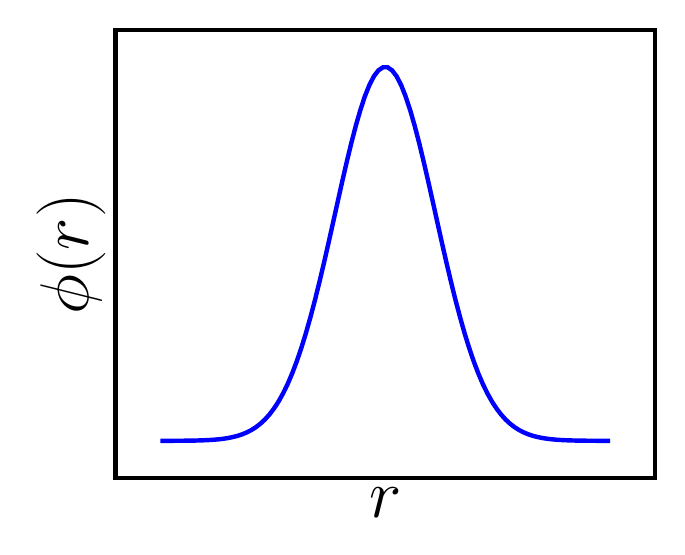
\begin{tikzpicture}
              \begin{axis}[ticks=none,samples=100,ylabel={\Huge $\phi(r)$},xlabel={\Huge $r$}, xlabel near ticks, ylabel near ticks, axis line style=ultra thick]
                \addplot[blue, ultra thick, domain=-1:1] {exp(-x^2*10)};
              \end{axis}
            \end{tikzpicture}
          }
        }
        \only<4,5>{\includesvg[width=\linewidth]{gfx/ibm_interp}}%
      \end{figure}
    }
    \only<3>{\centering Example: $\phi(r) \propto e^{-\frac{r^2}{2\sigma^2}}$}
    \end{column}
  \end{columns}
  \setbeamercovered{transparent=0}
  \onslide<2>{{\footnotesize Supervector notation $\vec{F} := \{\vec{F}_1,\dots,\vec{F}_N\}$}}
\end{frame}

\begin{frame}
  \frametitle{Particle-grid coupling}
  \framesubtitle{Performance}
  \centering
  \includesvg[width=0.35\columnwidth]{gfx/gridparticlesdense}
  \includegraphics[width=0.55\columnwidth]{gfx/ibm_comp_dens1_sorted_2080ti}
    \begin{center}
    \scriptsize 3D random distribution. Ran with a single RTX2080Ti GPU.
  \end{center}
\end{frame}

\section{The Force Coupling Method}
\begin{frame}
  \frametitle{Talk outline}
    \tableofcontents[
    sectionstyle=show/show,
    subsectionstyle=hide/hide/hide,
    subsubsectionstyle=hide/hide/hide/hide
    ]
\end{frame}
\begin{frame}
  \frametitle{Hydrodynamics}
  \framesubtitle{Algorithms for Brownian Dynamics with Hydrodynamic Interactions (BDHI)}
    \begin{figure}
    \centering
    \includesvg[width=0.55\linewidth]{gfx/multiscale}
  \end{figure}
  \note{
    \begin{itemize}
    \item And note that my contributions focus on the Smoluchowski level.
    \end{itemize}
  }
\end{frame}

\begin{frame}
  \frametitle{Complex fluids}
  \framesubtitle{The spatio-temporal landscape of numerical techniques.}
  \begin{figure}
    \centering    
    \begin{tikzpicture}
      \node[anchor=south west, inner sep=0] (image) {\includesvg[width=0.8\linewidth]{gfx/landscape}};
      \onslide<2>{
        \begin{scope}[shift={(image.south west)},x={(image.south east)},y={(image.north west)}]
        \filldraw[blue, opacity=0.6] (0.5,1) rectangle (0.72,0.07) node[midway] (A) {};\node[below=40pt of A, black, align=left]{\contourlength{1pt}\contour{white}{\textbf{Eulerian}}\\\contourlength{1pt}\contour{white}{\textbf{Lagrangian}}};
      \end{scope}
      }
    \end{tikzpicture}
    \caption{Figure courtesy of Rafael Delgado-Buscalioni.}
  \end{figure}
  \note{
    \begin{itemize}
    \item Which will require techniques that mix both continuous fields and particles.
    \end{itemize}
    }
\end{frame}


\subsection{Hydrodynamics}
\begin{frame}
  \frametitle{Smoluchowski level}
  \framesubtitle{Brownian Dynamics with Hydrodynamics Interactions (BDHI)}
  \Large
  \begin{equation*}
    d\vec{\ppos} = \tens{M}\vec{F}dt + \sqrt{2\kT\tens{M}}d\vec{\noise}
    + \kT\vec{\partial}_{\vec{\ppos}}\cdot\tens{M}dt.
  \end{equation*}
  \vspace*{10pt}
  \begin{overlayarea}{\linewidth}{0.6\paperheight}
    \only<1-3>{
      \begin{itemize}
      \item<1-> $\tens{M}(\vec{\ppos})$:\\
        Mobility tensor. Configuration- and BC-dependent
      \item<2-> $d\vec{\noise}$: Brownian motion
      \item<3-> $\kT\vec{\partial}_{\vec{\ppos}}\cdot\tens{M}dt$:\\
        Thermal drift. Zero depending on the BCs
      \end{itemize}
    }
    \only<4->{
      \centering \textbf{Problems}
      \vspace*{10pt}
      \begin{itemize}        
        \setlength\itemsep{10pt}
      \item<5-> $\tens{M}\vec{F}$: Matrix-vector multiplication is $O(N^2)$
      \item<6-> $\sqrt{\tens{M}}$: Quite expensive in general. $O(N^{[2.25-3]})$
      \item<7-> $\tens{M}$ might be unknown/not analytical.
      \end{itemize}
    }
  \end{overlayarea}
\end{frame}

\begin{frame}
  \frametitle{Hydrodynamics}
  \framesubtitle{Fluctuating Stokes equations}
  \begin{columns}[T]
    \begin{column}{0.34\linewidth}
      \begin{block}{Stokes equations}
        $%
        \begin{aligned}%
          \nabla \pi - \eta \nabla^2\vec{\fvel} &=  \vec{f} + \nabla\cdot \mathcal{Z}\\
          \nabla\cdot\vec{\fvel} &= 0%
        \end{aligned}
        $%
      \end{block}
      \onslide<2->{
        \begin{minipage}{\linewidth}
          \begin{block}{Fluid forcing}
            \centering $\vec{f}(\vec{r}) = \oper{S}(\vec{r})\vec{F}$
          \end{block}
          \begin{block}{Particle velocity}
            \centering $\vec{u}_i = \oper{J}_{\vec{q}_i}\vec{v}(\vec{r})$
          \end{block}
        \end{minipage}
      }
      \end{column}
      \begin{column}{0.63\linewidth}
        \onslide<3->{
          {
            \begin{center}
              \huge \textbf{Green formalism}
            \end{center}
          }
          \centering $\vec{v}(\vec{r}) = \oper{G}\tilde{\vec{f}}
          \onslide<4->{
            :=\int{\oper{G}(\vec{r}, \vec{r}^\prime)\tilde{\vec{f}}(\vec{r}^\prime) d\vec{r}^\prime}
          }$ %\left(\oper{S}\vec{F} + \nabla\cdot\mathcal{Z}\right)$$
          \onslide<5->{
            \begin{block}{Force Coupling Method (FCM)}
              \centering $\frac{d\vec{q}_i}{dt} = \vec{u}_i = \oper{J}_{\vec{\ppos}_i}\oper{G}(\oper{S}\vec{F} + \nabla\cdot\mathcal Z)$
            \end{block}
          }%
          \begin{overlayarea}{\linewidth}{0.3\paperheight}
            \only<6>{
                \begin{equation*}
                \begin{aligned}
                  &\tens{M} &=&\oper{J}\oper{G}\oper{S}\\
                  &\tens{M}^{1/2} &=&\oper{J}\oper{G}\nabla\cdot\\
                  &\vec{\partial}_{\vec{q}}\cdot\tens{M} &=&0\leftarrow \text{Incompressible}
                \end{aligned}
              \end{equation*}
            }%
            \only<7>{
              \begin{equation*}
                \tens{M}_{ij}=\iint{\delta_a(\vec{r}-\vec{\ppos}_j)\oper{G}(\vec{r},\vec{r}^\prime)\delta_a(\vec{\ppos}_i-\vec{r}^\prime)d\vec{r}^\prime d\vec{r}}
              \end{equation*}
            }%
            \onslide<8->{\centering $\oper{G} :=-\eta^{-1}\nabla^{-2}\left(\mathbb{I} - \nabla\nabla^{-2}\nabla\right)$\\}%
            \onslide<9>{
              \begin{block}{\centering Open boundaries}
                \centering $\oper{G}\rightarrow \tens{O}(\vec{r}) = \frac{1}{8\pi\eta r}\left(\mathbb{I} - \frac{\vec{r}\otimes\vec{r}}{r^2}\right)$
              \end{block}
            }
          \end{overlayarea}
        }
      \end{column}
    \end{columns}
  \end{frame}

\begin{frame}
  \frametitle{Hydrodynamics}
  \framesubtitle{Triply periodic FCM}
  \begin{overprint}
    \huge
    \begin{equation*}
    \tikz[baseline, remember picture]{\node[anchor=base] (a) {$\vec{u}_i= \oper{J}_{\vec{\ppos}_i}\oper{G}(\oper{S}\vec{F} + \nabla\cdot\mathcal Z)$};}
  \end{equation*}
  \vspace*{50pt}
  \onslide<2->{
        \begin{equation*}
        \tikz[baseline, remember picture]{ \node[anchor=base] (b) {$\vec{u}_i = \oper{J}_{\vec{\ppos}_i}\onslide<3>{\mathfrak{F}^{-1}}\only<3>{\fou{\oper{G}}}\only<2>{\oper{G}}(\onslide<3>{\mathfrak{F}}\oper{S}\vec{F} + \onslide<2>{\nabla}\onslide<3>{\vec{k}}\cdot\mathcal Z\onslide<3>{_{\vec{k}}})$};}
      \end{equation*}
      \begin{tikzpicture}[overlay, remember picture]
        \path[very thick, -Triangle, line width=3pt] (a) edge node[midway, above right] {$\mathfrak{F}$: Fourier transform} (b);
      \end{tikzpicture}
    }
  \end{overprint}
\end{frame}

\begin{frame}
  \frametitle{Hydrodynamics}
  \framesubtitle{Triply periodic FCM}
  \begin{block}{\huge\centering Force Coupling Method}
    \huge\centering$\vec{u}_i = \oper{J}_{\vec{\ppos}_i}\mathfrak{F}^{-1}\fou{\oper{G}}(\mathfrak{F}\oper{S}\vec{F} + \vec{k}\cdot\mathcal Z_{\vec{k}})$
  \end{block}
  \begin{block}{\huge\centering Triply Periodic}
    \huge\centering $\fou{\oper{G}}_{\text{3D}} :=\eta^{-1}k^{-2}\left(\mathbb{I} - \frac{\vec{k}\otimes\vec{k}}{k^2}\right)$
  \end{block}
\end{frame}

\begin{frame}
  \frametitle{Hydrodynamics in confined geometries}
  \framesubtitle{New algorithms for Brownian Dynamics with Hydrodynamic Interactions (BDHI)}
   \begin{block}{\centering Force Coupling Method}
      \begin{center}
        \Large $\vec{u}_i = \oper{J}_{\vec{\ppos}_i}\mathfrak{F}^{-1}\fou{\oper{G}}_\text{\tiny 3D}\big(\mathfrak{F}\oper{S}\vec{F} + \vec{k}\cdot\mathcal Z\big)$
      \end{center}
   \end{block}
  \begin{columns}[T]
    \begin{column}{0.5\linewidth}
      \begin{itemize}
      \item<1-> Quasi two-dimensional (q2D)
      \end{itemize}
      \begin{overlayarea}{\linewidth}{0.5\paperheight}
        \includesvg[width=0.9\linewidth]{gfx/q2d}\\
          \begin{center}
            q2D: $\delta\rightarrow 0$.\\3D fluid, 2D particles
          \end{center}
         \end{overlayarea}
    \end{column}
    \begin{column}{0.5\linewidth}
      \begin{itemize}
      \item Doubly Periodic Stokes (DPStokes)
      \end{itemize}
      \includesvg[width=\linewidth]{gfx/dpstokes_sketch}
    \end{column}
  \end{columns}
  \begin{center}
    \vspace*{-6pt}
    \small[{\bf Raul P. Pelaez} et. al. JSTAT 2018.]     \small [O. Maxian, {\bf Raul P. Pelaez} et. al. J. Chem. Phys. 2021.]
  \end{center}
\end{frame}


\subsection{Electrostatics}
\begin{frame}
  \frametitle{Triply Periodic Electrostatics}
  \framesubtitle{Force Coupling Method for the Poisson equation}
  \begin{center}
    \begin{minipage}{0.7\linewidth}    
      \begin{block}{Poisson}
        \Large \centering $\varepsilon_0\nabla^2\phi = -f(\vec{r}) = -\oper{S}(\vec{r})\vec{Q}$
      \end{block}
    \end{minipage}
  \end{center}
  \begin{overlayarea}{\linewidth}{0.5\paperheight}
    \begin{columns}[T]
      \begin{column}{0.39\linewidth}
        \begin{block}{Spreading}
          \centering $\oper{S}(\vec{r})\vec{Q} = \sum_i Q_i \delta_a(\vec{\ppos}_i - \vec{r})$
        \end{block}
        \begin{block}{Gaussian sources}
          \centering$\delta_a(\vec{r})\propto e^{-r^2/(2a^2)}$
        \end{block}        
      \end{column}
      \begin{column}{0.59\linewidth}
          \begin{equation*}
            \vec{E}(\vec{\fpos}) = \partial_{\vec{\fpos}}\phi \rightarrow \fou{\vec{E}} = i\vec{k}\fou{\phi}
          \end{equation*}
          \begin{equation*}
            \vec{F}_i = Q_i\oper{J}_{\vec{\ppos}_i}\vec{E}(\vec{r})
          \end{equation*}
        \begin{block}{Charges to forces}
          \centering \Large $\vec{F}_i = Q_i\oper{J}_{\vec{q}_i}\mathfrak{F}^{-1}i\vec{k}\fou{\oper{G}}_P\mathfrak{F}\oper{S}\vec{Q}$
        \end{block}
        $$\fou{\oper{G}}_P = \left(\varepsilon_0 k^2\right)^{-1}$$
      \end{column}
    \end{columns}
  \end{overlayarea}
  \footnotesize Supervector notation. Charges $\vec{Q} := \{Q_1,\dots,Q_N\}$
  \begin{center}
    \small [O. Maxian, {\bf Raul P. Pelaez} et. al. J. Chem. Phys. 2021.]
  \end{center}
\end{frame}

\section{UAMMD}
\begin{frame}
  \frametitle{Talk outline}
  \tableofcontents[
  sectionstyle=show/shaded,
  subsectionstyle=show/show/hide,
  subsubsectionstyle=show/show/show/hide
  ]
  \note{In this final section I will introduce UAMMD, the GPU software framework for complex fluids that encases, among others, all the algorithms I have previously introduced.}
\end{frame}

\begin{frame}
  \frametitle{Universally Adaptable Multiscale Molecular Dynamics}
  \framesubtitle{What makes UAMMD stand out}
  \Large
  \begin{center}
    UAMMD: A CUDA/C++ library for complex fluids.
    \rule{0.7\textwidth}{1.4pt}
  \end{center}
  \begin{itemize}
  \item<1-> Header only and library-like
  \item<2-> Lightweight with minimal dependencies
  \item<3-> Hackable
  \item<4-> Focus on hydrodynamics
  \end{itemize}
\end{frame}

\subsection{Basic code structure}
\begin{frame}[fragile]
  \frametitle{UAMMD}
  \framesubtitle{Conceptual hierarchy}
  \includesvg[width=\linewidth]{gfx/sketchUAMMD}
  \begin{overprint}
    \onslide<1>
    \begin{block}{\centering \Large Remember}
      \centering \Large ``Interacting \emph{particles} with a state that \emph{evolves}''
    \end{block}
    \onslide<2>
    \begin{code2}[]{label=code:module}
      #include<uammd.cuh>
      int main(int argc, char* argv[]){
        auto sys = std::make_shared<System>(argc, argv);
        ...
    \end{code2}
    \onslide<3>
    \begin{code2}[]{label=code:module}
      #include<uammd.cuh>
      int main(int argc, char* argv[]){
        auto sys = std::make_shared<System>(argc, argv);
        const int nP = 1e6; //Number of particles
        auto pd = std::make_shared<ParticleData>(nP, sys);
        ...
      \end{code2}
      \onslide<4>
    \begin{code2}[]{label=code:module}
      ...
      auto pos = pd->getPos(access::cpu, access::write);
      pos[0] = {1,1,1,0}; // x,y,x, color (type)
      ...
    \end{code2}
    \onslide<5>
    \begin{code2}[]{label=code:module}
      ...
      auto bd = std::make_shared<BDHI::FCM>(pd, /*Parameters*/);
      bd->forwardTime(); //Exposed by every Integrator
      ...      
    \end{code2}
    \onslide<6>
    \begin{code2}[]{label=code:module}
      ...
      auto elec = std::make_shared<Poisson>(pd,/*Parameters*/);
      elec->sum({.force=true, .energy=false, .virial=false});
      //Exposed by every Integrator
      bd->addInteractor(elec);
      bd->forwardTime();
      ...      
    \end{code2}
  \end{overprint}
\end{frame}
  
\begin{frame}
  \frametitle{Available solvers}
  \includesvg[width=\linewidth]{gfx/sketchUAMMD_integrators}
\end{frame}

\begin{frame}
  \frametitle{Available interactions}
  \includesvg[width=\linewidth]{gfx/sketchUAMMD_interactors}
\end{frame}

\begin{frame}
  \frametitle{UAMMD's online presence}
  \framesubtitle{Git repository}
  {\centering {\color{blue} \url{https://github.com/RaulPPelaez/uammd}}}
  \begin{figure}
    \centering
    \only<1>{\includegraphics[height=0.7\paperheight]{gfx/uammdgithub}}
    \only<2-3>{
      \onslide<3->{\includegraphics[height=0.7\paperheight]{gfx/uammdtutorial1}}
      \onslide<2->{\includegraphics[height=0.7\paperheight]{gfx/uammdexamples}}
    }
    \only<4>{
      \onslide<4->{\includegraphics[height=0.7\paperheight]{gfx/uammdtutorial1}}
      \onslide<4->{\includegraphics[height=0.7\paperheight]{gfx/uammdtutorial2}}
    }
  \end{figure}
\end{frame}

\begin{frame}
  \frametitle{UAMMD's online presence}
  \framesubtitle{Documentation}
  {\centering {\color{blue} \url{https://uammd.readthedocs.io}}}
  \begin{figure}
    \centering
    \includegraphics[height=0.7\paperheight]{gfx/uammdreadthedocs}
  \end{figure}
\end{frame}

\section{Examples}
\begin{frame}
  \frametitle{Talk outline}
    \tableofcontents[
    sectionstyle=show/show,
    subsectionstyle=hide/hide/hide,
    subsubsectionstyle=hide/hide/hide/hide
    ]
\end{frame}


\begin{frame}[fragile]
  \frametitle{Lets clone}
  \begin{center}
    \Large
    \begin{codebash}[]{label=code:bash1}
      $ git clone git@github.com:RaulPPelaez/2022Bilbao
    \end{codebash}
  \end{center}
\end{frame}


\begin{frame}[fragile]
  \frametitle{The falling logo}
  \begin{center}
    \includegraphics[height=0.7\paperheight]{gfx/poster}
  \end{center}
\end{frame}

\begin{frame}[fragile]
  \frametitle{Particle-grid coupling}
  \begin{columns}[T]
    \begin{column}{0.5\linewidth}
      \includesvg[width=\columnwidth]{gfx/gridparticles}
    \end{column}
    \begin{column}{0.3\linewidth}
      $\vec{f}(\vec{r}) = \oper{S}(\vec{r})\vec{F}$
      \includesvg[width=0.9\columnwidth]{gfx/ibm_spread}
      $\vec{u}_i = \oper{J}_{\vec{q}_i}\vec{v}(\vec{r})$
      \includesvg[width=0.9\columnwidth]{gfx/ibm_interp}
    \end{column}
  \end{columns}
\end{frame}




\begin{frame}
  \begin{center}
    \Huge Thanks for your attention!
  \end{center}
\end{frame}
\end{document}
%%% Local Variables: 
%%% TeX-command-extra-options: "-shell-escape"
%%% End: